%%%%%%%%%%%%%%%%%%%%%%%%%%%%%%%%%%%%%%%%%%%%%%%%%%%%%%%%%%%%%%%%%%%%%%%%%%%%%%%%%%
\begin{frame}[fragile]\frametitle{}
\begin{center}
{\Large Equations}
\end{center}
\end{frame}

%%%%%%%%%%%%%%%%%%%%%%%%%%%%%%%%%%%%%%%%%%%%%%%%%%%%%%%%%%%
 \begin{frame}[fragile]\frametitle{Algebra}
\begin{itemize}
\item Equation 'equates' two expressions. E.g. $3x+4=10$
\item We solve equations for unknowns such as $x$
\item $x$ in the equation above have coefficient $3$.
\item Others like $4$ and $10$ are constants.
\end{itemize}
\end{frame}

%%%%%%%%%%%%%%%%%%%%%%%%%%%%%%%%%%%%%%%%%%%%%%%%%%%%%%%%%%%
 \begin{frame}[fragile]\frametitle{Equations}
 $3x+4=10$
\begin{itemize}
\item To Solve, we isolate $x$ on one side by operations.
\item $3x + 4 - 4 = 10 - 4$
\item Although a short hand way is just to transfer $4$ from one side to other and changing the sign.
\item $3x = 6$
\item In case of coefficients, you divide after crossing the $=$
\item $3x/3 = 6/3$
\item $x = 2$
\item To test, plug $x=2$, back in the original equation and see if both sides 'equate'.
\end{itemize}
\end{frame}

%%%%%%%%%%%%%%%%%%%%%%%%%%%%%%%%%%%%%%%%%%%%%%%%%%%%%%%%%%%
 \begin{frame}[fragile]\frametitle{The Distributive Property}
 
\begin{itemize}
\item $3(x+2)=18$ is same as $3x + 6 = 18$
\item Intuitively we multiply everything from outside, as if its a coefficient.
\item Now instead of just 3 I have another expression to multiply $(3x + 3)(x+2) = 18$
\item Same distributive property works?
\end{itemize}
\end{frame}

%%%%%%%%%%%%%%%%%%%%%%%%%%%%%%%%%%%%%%%%%%%%%%%%%%%%%%%%%%%
 \begin{frame}[fragile]\frametitle{Two Variables}
 
\begin{itemize}
\item $2y - 4x = 2$
\item How to solve?
\item Can we solve?
\end{itemize}
\end{frame}

%%%%%%%%%%%%%%%%%%%%%%%%%%%%%%%%%%%%%%%%%%%%%%%%%%%%%%%%%%%
 \begin{frame}[fragile]\frametitle{Two Variables}
 
\begin{itemize}
\item $2y - 4x = 2$
\item Isolate $y$ first 
\item $2y = 2 + 4x$
\item $y = 1 + 2x$
\item Thats y's definition in terms of x.
\item For any x, y can be calculated.
\item x, y if plotted form a line, thus the original equation is called as Linear Equation.
\end{itemize}
\end{frame}

%%%%%%%%%%%%%%%%%%%%%%%%%%%%%%%%%%%%%%%%%%%%%%%%%%%%%%%%%%%
 \begin{frame}[fragile]\frametitle{Line Plot}
 
\begin{itemize}
\item X intercept is where line crosses x axis, where y is 0 (put in the eqn)
\item Y intercept is where line crosses y axis, where x is 0 (put in the eqn)
\end{itemize}
\begin{center}
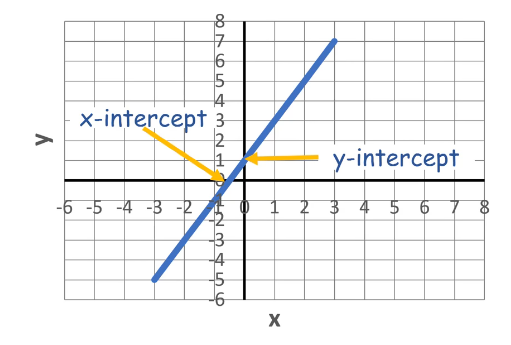
\includegraphics[width=0.5\linewidth,keepaspectratio]{lineqn}
\end{center}
\end{frame}


%%%%%%%%%%%%%%%%%%%%%%%%%%%%%%%%%%%%%%%%%%%%%%%%%%%%%%%%%%%
 \begin{frame}[fragile]\frametitle{Line Plot}
 
\begin{itemize}
\item Slope is change in y per change in x
\item Calculated using any two points.
\item Slope-Intercept form is $y = mx + b$
\end{itemize}
\begin{center}
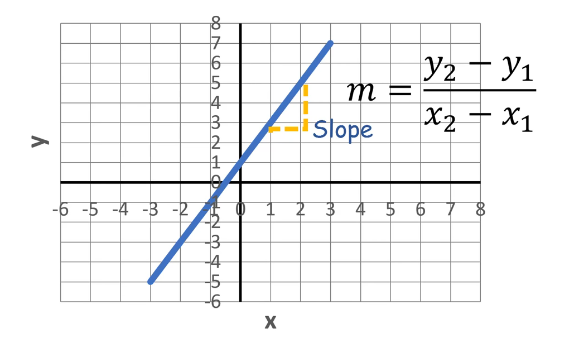
\includegraphics[width=0.5\linewidth,keepaspectratio]{lineqn1}
\end{center}
\end{frame}

%%%%%%%%%%%%%%%%%%%%%%%%%%%%%%%%%%%%%%%%%%%%%%%%%%%%%%%%%%%
 \begin{frame}[fragile]\frametitle{Exercise}
Find slope and both intercepts of $2y + 3 = 3x -1 $
\end{frame}

%%%%%%%%%%%%%%%%%%%%%%%%%%%%%%%%%%%%%%%%%%%%%%%%%%%%%%%%%%%
 \begin{frame}[fragile]\frametitle{Exercise}
\begin{lstlisting}
import pandas as pd

# Create a dataframe with an x column containing values from -10 to 10
df = pd.DataFrame ({'x': range(-10, 11)})

# Add a y column by applying the solved equation to x
df['y'] = (3*df['x'] - 4) / 2

print(df)
\end{lstlisting}
\end{frame}

%%%%%%%%%%%%%%%%%%%%%%%%%%%%%%%%%%%%%%%%%%%%%%%%%%%%%%%%%%%
 \begin{frame}[fragile]\frametitle{Exercise}
\begin{lstlisting}
from matplotlib import pyplot as plt

plt.plot(df.x, df.y, color="grey", marker = "o")
plt.xlabel('x')
plt.ylabel('y')
plt.grid()
plt.show()
\end{lstlisting}
\begin{center}
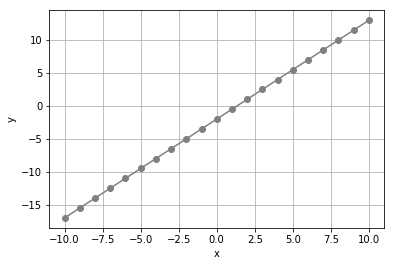
\includegraphics[width=0.5\linewidth,keepaspectratio]{lineqn2}
\end{center}
\end{frame}


%%%%%%%%%%%%%%%%%%%%%%%%%%%%%%%%%%%%%%%%%%%%%%%%%%%%%%%%%%%
 \begin{frame}[fragile]\frametitle{System of Equations}
 9 items cost 75c, how many are apples and how many oranges?
\begin{center}
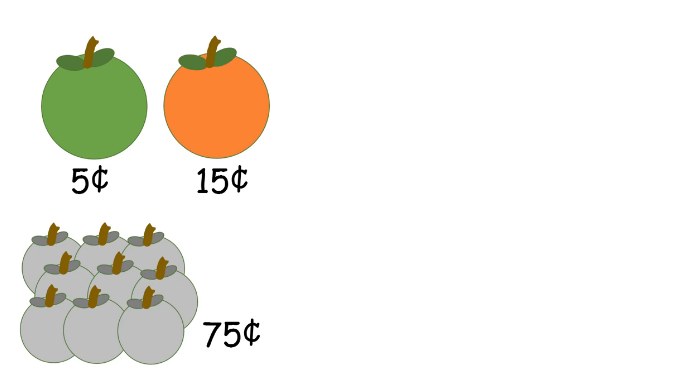
\includegraphics[width=0.5\linewidth,keepaspectratio]{lineqn3}

{\tiny (Ref: Essentials of Mathematics - DAT 256 EdX)}
\end{center}
\end{frame}

%%%%%%%%%%%%%%%%%%%%%%%%%%%%%%%%%%%%%%%%%%%%%%%%%%%%%%%%%%%
 \begin{frame}[fragile]\frametitle{System of Equations}
Let number of apples be x and oranges be y.
\begin{center}
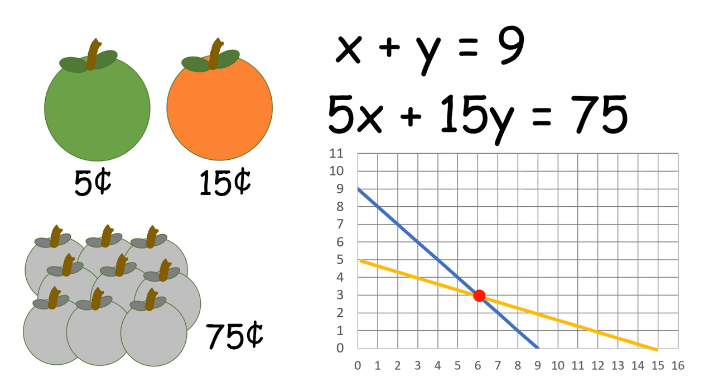
\includegraphics[width=0.5\linewidth,keepaspectratio]{lineqn4}

{\tiny (Ref: Essentials of Mathematics - DAT 256 EdX)}
\end{center}
Blue line represents $x+y=9$ and yellow line $5x+15y=75$. Their intersection, the common point shared by two equations, is the solution.
\end{frame}

%%%%%%%%%%%%%%%%%%%%%%%%%%%%%%%%%%%%%%%%%%%%%%%%%%%%%%%%%%%
 \begin{frame}[fragile]\frametitle{System of Equations}
System of Linear equations can be solved, apart from line intersection method, by elimination method.
\begin{center}
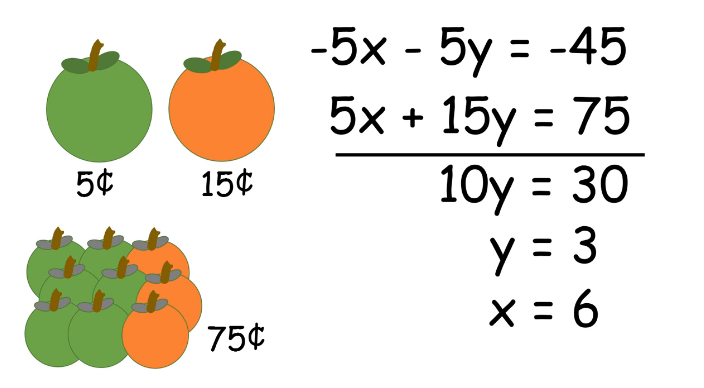
\includegraphics[width=0.5\linewidth,keepaspectratio]{lineqn5}

{\tiny (Ref: Essentials of Mathematics - DAT 256 EdX)}
\end{center}
Make one of the equations (say, first) as NEGATIVE of the other in one variable, so that their addition cancels it out, leaving only one variable. Easy to find solution. Put that value back in the original equation, to get the other variable value.
\end{frame}

%%%%%%%%%%%%%%%%%%%%%%%%%%%%%%%%%%%%%%%%%%%%%%%%%%%%%%%%%%%
 \begin{frame}[fragile]\frametitle{Exercise}
Solve $x + y = 16$ and $10x + 25y = 250$
\end{frame}





%%%%%%%%%%%%%%%%%%%%%%%%%%%%%%%%%%%%%%%%%%%%%%%%%%%%%%%%%%%%%%%%%%%%%%%%%%%%%%%%%%
\begin{frame}[fragile]\frametitle{}
\begin{center}
{\Large Polynomials}
\end{center}
\end{frame}



%%%%%%%%%%%%%%%%%%%%%%%%%%%%%%%%%%%%%%%%%%%%%%%%%%%%%%%%%%%
 \begin{frame}[fragile]\frametitle{Polynomials}
\begin{itemize}
\item Polynomials = Many (Poly) terms
\item Terms can be constants, coefficients with variables, some with exponentials
\item $6 + 4x - 3 x^2$
\item Any arithmetic operators can be used
\item Standard form is in decreasing powers $-3x^2 + 4x + 6$
\end{itemize}
\end{frame}

%%%%%%%%%%%%%%%%%%%%%%%%%%%%%%%%%%%%%%%%%%%%%%%%%%%%%%%%%%%
 \begin{frame}[fragile]\frametitle{Polynomial Operations}
Addition or subtraction of polynomials is those operations on similar exponential terms
\begin{center}
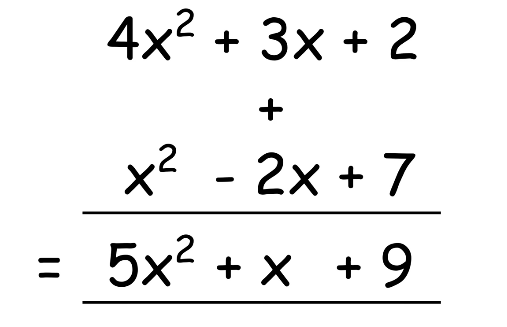
\includegraphics[width=0.6\linewidth,keepaspectratio]{polyadd}
\end{center}
\end{frame}


%%%%%%%%%%%%%%%%%%%%%%%%%%%%%%%%%%%%%%%%%%%%%%%%%%%%%%%%%%%
 \begin{frame}[fragile]\frametitle{Polynomial Operations}
For multiplication, each term in first is multiplied with all in the second, then added.
\begin{center}
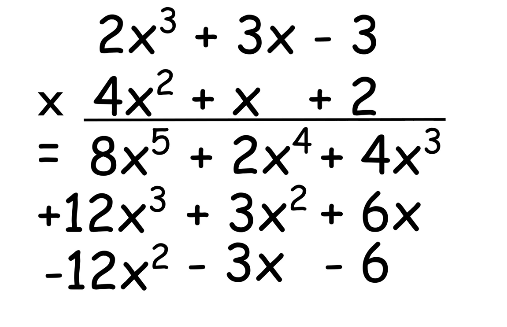
\includegraphics[width=0.6\linewidth,keepaspectratio]{polymul}
\end{center}
$8x^5 + 2x^4 + 16x^3-9x^2+3x-6$
\end{frame}

%%%%%%%%%%%%%%%%%%%%%%%%%%%%%%%%%%%%%%%%%%%%%%%%%%%%%%%%%%%
 \begin{frame}[fragile]\frametitle{Polynomial Operations}
Division by a single term
\begin{center}
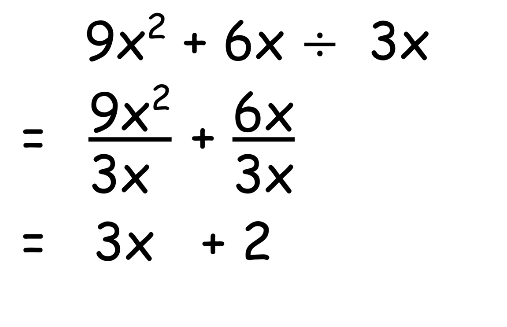
\includegraphics[width=0.6\linewidth,keepaspectratio]{polydiv}
\end{center}
\end{frame}

%%%%%%%%%%%%%%%%%%%%%%%%%%%%%%%%%%%%%%%%%%%%%%%%%%%%%%%%%%%
 \begin{frame}[fragile]\frametitle{Polynomial Operations}
Division by a complex term. Find the factor with highest power term, subtract, repeat on remainder.
\begin{center}
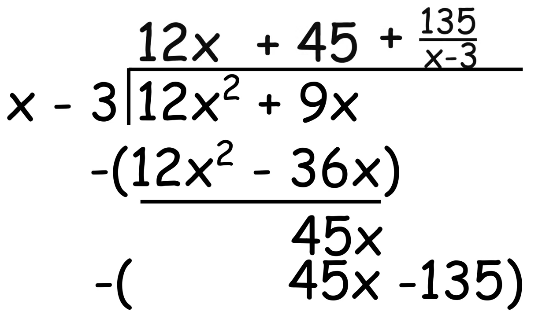
\includegraphics[width=0.6\linewidth,keepaspectratio]{polydiv1}
\end{center}
\end{frame}

%%%%%%%%%%%%%%%%%%%%%%%%%%%%%%%%%%%%%%%%%%%%%%%%%%%%%%%%%%%%%%%%%%%%%%%%%%%%%%%%%%
\begin{frame}[fragile]\frametitle{}
\begin{center}
{\Large Factorization}
\end{center}
\end{frame}



%%%%%%%%%%%%%%%%%%%%%%%%%%%%%%%%%%%%%%%%%%%%%%%%%%%%%%%%%%%
 \begin{frame}[fragile]\frametitle{Factors}
\begin{itemize}
\item Restating expression in terms of multiplication of multiple expressions.
\item Eg $6 = 1 \times 6 = 2 \times 3$
\item 1,2,3,6 are factors of 6
\item Similarly $1x,2x,3x,6x$ are factors of $6x^2$
\item What are common factors of 6 and 15?
\item 1 and 3. 
\item 3 is GCF  (Greatest Common Factor )
\item ma saa vii : mahattam samanya vibhajak
\end{itemize}
\end{frame}

%%%%%%%%%%%%%%%%%%%%%%%%%%%%%%%%%%%%%%%%%%%%%%%%%%%%%%%%%%%
 \begin{frame}[fragile]\frametitle{Simplifying Polynomials}
\begin{itemize}
\item GCF of $12x$ and $20x^2$ ?
\item GCF of coefficients into lowest variable power term ie $4x$
\item Useful in simplifying Polynomials
\item $9x + 12y$
\item GCF is 3
\item $= 3(3x) + 3(4y) = 3(3x+4y)$
\end{itemize}
\end{frame}

%%%%%%%%%%%%%%%%%%%%%%%%%%%%%%%%%%%%%%%%%%%%%%%%%%%%%%%%%%%%%%%%%%%%%%%%%%%%%%%%%%
\begin{frame}[fragile]\frametitle{}
\begin{center}
{\Large Quadratic Equations}
\end{center}
\end{frame}

%%%%%%%%%%%%%%%%%%%%%%%%%%%%%%%%%%%%%%%%%%%%%%%%%%%%%%%%%%%
 \begin{frame}[fragile]\frametitle{Quadratic Equations}
 Highest order term is Square.e.g Parabola is open at top, closed at bottom.
\begin{center}
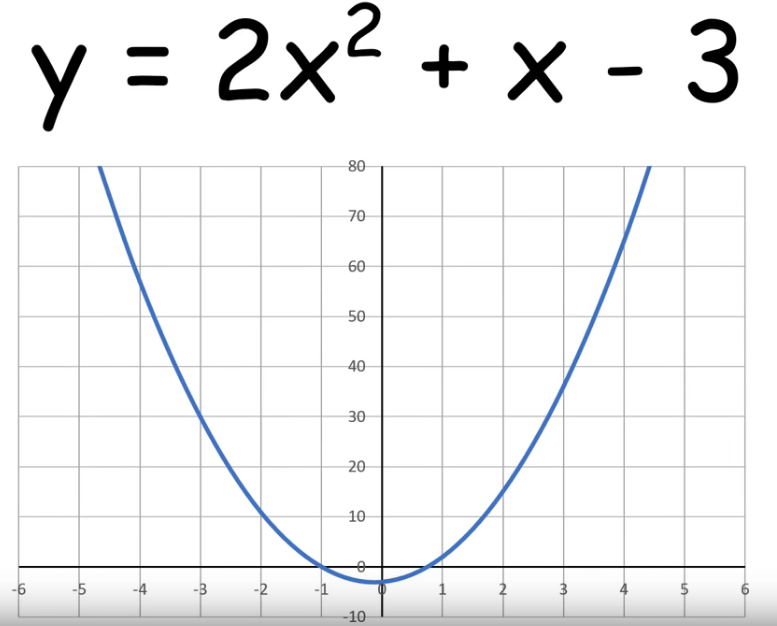
\includegraphics[width=0.6\linewidth,keepaspectratio]{para1}
\end{center}

\end{frame}


%%%%%%%%%%%%%%%%%%%%%%%%%%%%%%%%%%%%%%%%%%%%%%%%%%%%%%%%%%%
 \begin{frame}[fragile]\frametitle{Quadratic Equations}
With negative highest term similar Parabola is open at bottom, closed at top.
\begin{center}
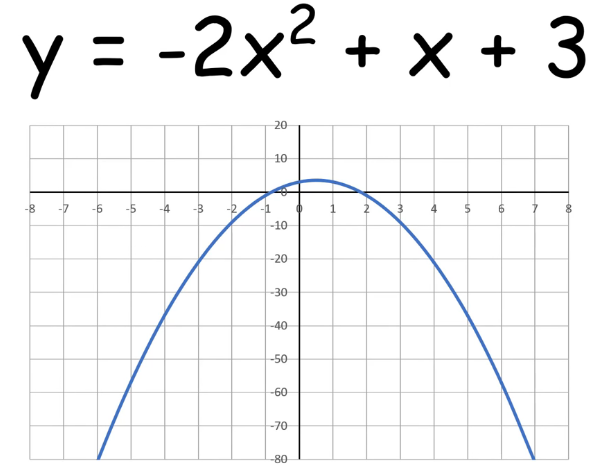
\includegraphics[width=0.6\linewidth,keepaspectratio]{para2}
\end{center}

\end{frame}

%%%%%%%%%%%%%%%%%%%%%%%%%%%%%%%%%%%%%%%%%%%%%%%%%%%%%%%%%%%
 \begin{frame}[fragile]\frametitle{Exercise}
$y = 2x^2 + 2x - 4$

\begin{lstlisting}
import pandas as pd

# Create a dataframe with an x column containing values to plot
df = pd.DataFrame ({'x': range(-9, 9)})

# Add a y column by applying the quadratic equation to x
df['y'] = 2*df['x']**2 + 2 *df['x'] - 4

# Plot the line
%matplotlib inline
from matplotlib import pyplot as plt

plt.plot(df.x, df.y, color="grey")
plt.xlabel('x')
plt.ylabel('y')
plt.grid()
plt.axhline()
plt.axvline()
plt.show()
\end{lstlisting}
\end{frame}

%%%%%%%%%%%%%%%%%%%%%%%%%%%%%%%%%%%%%%%%%%%%%%%%%%%%%%%%%%%
 \begin{frame}[fragile]\frametitle{Quadratic Equations}
\begin{center}
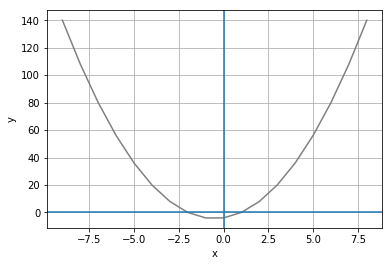
\includegraphics[width=0.6\linewidth,keepaspectratio]{para3}
\end{center}

\end{frame}

